\documentclass[border=4pt]{standalone}
\usepackage{pgfplots}
\usepgfplotslibrary{groupplots}
\pgfplotsset{compat=1.17}
\begin{document}
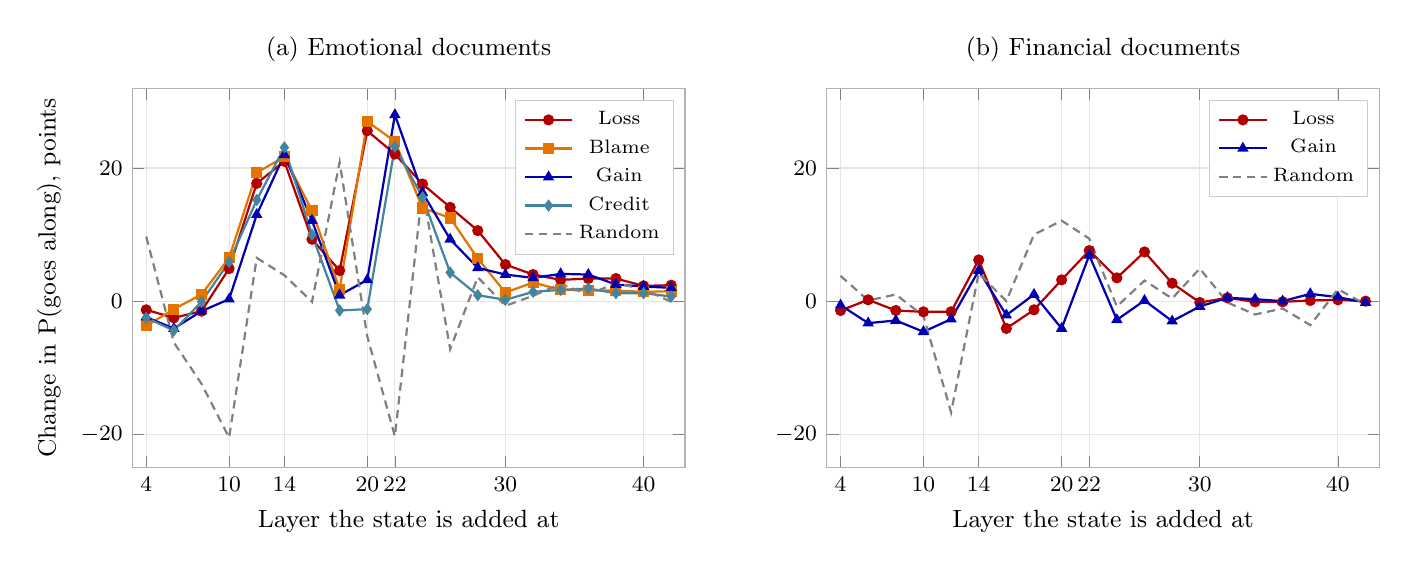
\begin{tikzpicture}
\begin{groupplot}[
  group style={group size=2 by 1, horizontal sep=1.8cm},
  width=8.6cm, height=6.4cm, xmin=3, xmax=43, xtick={4,10,14,20,22,30,40},
  ymajorgrids, xmajorgrids, grid style={gray!20}, axis line style={gray!60},
  tick label style={font=\footnotesize}, label style={font=\small},
  title style={font=\small, align=center}, xlabel={Layer the state is added at},
  legend style={font=\scriptsize, draw=gray!40, at={(0.98,0.97)}, anchor=north east, legend columns=1}]
\nextgroupplot[ylabel={Change in P(goes along), points}, ymin=-25, ymax=32, title={(a) Emotional documents}]
\addplot[color=red!70!black, thick, mark=*, mark size=1.6pt] coordinates {(4,-1.3) (6,-2.5) (8,-1.5) (10,4.9) (12,17.7) (14,21.0) (16,9.3) (18,4.6) (20,25.6) (22,22.1) (24,17.6) (26,14.1) (28,10.6) (30,5.5) (32,4.0) (34,3.2) (36,3.4) (38,3.4) (40,2.3) (42,2.4)};
\addplot[color=orange!90!black, thick, mark=square*, mark size=1.6pt] coordinates {(4,-3.7) (6,-1.2) (8,1.0) (10,6.5) (12,19.3) (14,21.7) (16,13.6) (18,1.8) (20,27.0) (22,24.0) (24,14.0) (26,12.5) (28,6.4) (30,1.3) (32,2.8) (34,1.7) (36,1.6) (38,1.6) (40,1.4) (42,1.5)};
\addplot[color=blue!70!black, thick, mark=triangle*, mark size=1.6pt] coordinates {(4,-2.4) (6,-4.1) (8,-1.5) (10,0.3) (12,13.0) (14,22.0) (16,12.1) (18,0.9) (20,3.2) (22,28.0) (24,16.3) (26,9.3) (28,5.0) (30,4.0) (32,3.5) (34,4.1) (36,4.0) (38,2.5) (40,2.2) (42,2.0)};
\addplot[color=cyan!60!black, thick, mark=diamond*, mark size=1.6pt] coordinates {(4,-2.5) (6,-4.4) (8,-0.1) (10,5.9) (12,15.2) (14,23.1) (16,10.0) (18,-1.4) (20,-1.2) (22,23.2) (24,15.6) (26,4.3) (28,0.9) (30,0.2) (32,1.4) (34,1.7) (36,1.9) (38,1.2) (40,1.2) (42,0.7)};
\addplot[color=gray, thick, mark=none, densely dashed, mark size=1.6pt] coordinates {(4,9.7) (6,-6.2) (8,-12.4) (10,-20.5) (12,6.5) (14,3.9) (16,-0.1) (18,20.9) (20,-5.3) (22,-20.3) (24,16.8) (26,-7.2) (28,3.6) (30,-0.7) (32,0.8) (34,2.6) (36,1.0) (38,2.7) (40,1.8) (42,-0.1)};
\legend{Loss, Blame, Gain, Credit, Random}
\nextgroupplot[ymin=-25, ymax=32, title={(b) Financial documents}]
\addplot[color=red!70!black, thick, mark=*, mark size=1.6pt] coordinates {(4,-1.4) (6,0.2) (8,-1.4) (10,-1.6) (12,-1.6) (14,6.2) (16,-4.1) (18,-1.3) (20,3.2) (22,7.6) (24,3.5) (26,7.4) (28,2.7) (30,-0.2) (32,0.5) (34,-0.1) (36,-0.1) (38,0.1) (40,0.2) (42,0.0)};
\addplot[color=blue!70!black, thick, mark=triangle*, mark size=1.6pt] coordinates {(4,-0.6) (6,-3.3) (8,-2.9) (10,-4.6) (12,-2.7) (14,4.6) (16,-2.1) (18,1.0) (20,-4.1) (22,6.9) (24,-2.8) (26,0.1) (28,-3.0) (30,-0.8) (32,0.5) (34,0.3) (36,-0.0) (38,1.1) (40,0.6) (42,-0.2)};
\addplot[color=gray, thick, mark=none, densely dashed, mark size=1.6pt] coordinates {(4,3.8) (6,0.1) (8,1.0) (10,-2.2) (12,-16.7) (14,4.2) (16,-0.0) (18,10.0) (20,12.1) (22,9.4) (24,-0.8) (26,3.1) (28,0.4) (30,4.9) (32,-0.2) (34,-2.0) (36,-1.1) (38,-3.6) (40,1.8) (42,-0.5)};
\legend{Loss, Gain, Random}
\end{groupplot}
\end{tikzpicture}
\end{document}
